\documentclass[aspectratio=169,10pt]{beamer}
% =====================================================================
% pyflightstream User Guide
% Didactic material: requirements, architecture, examples, and the
% step by step recipes for every supported simulation type.
% Geovana Neves
% Note: no em dashes or en dashes are used anywhere in this document.
% The built pdf never enters Git (repository guard); build locally
% with scripts/build-guide.ps1.
% =====================================================================
\usetheme{Madrid}
\usecolortheme{default}
\usepackage[T1]{fontenc}
\usepackage[utf8]{inputenc}
\usepackage{amsmath,amssymb}
\usepackage{booktabs}
\usepackage{graphicx}
\usepackage{listings}
\usepackage{tikz}
\usepackage{pgfplots}
\pgfplotsset{compat=1.17}
\usetikzlibrary{arrows.meta,positioning,calc,shapes.geometric}

% ---- Color palette -------------------------------------------------
\definecolor{deepblue}{RGB}{18,58,102}
\definecolor{accentteal}{RGB}{0,124,146}
\definecolor{accentorange}{RGB}{200,90,20}
\definecolor{softgray}{RGB}{240,242,245}
\definecolor{statusgreen}{RGB}{26,110,47}
\definecolor{statusblue}{RGB}{20,80,138}
\definecolor{statusred}{RGB}{163,48,48}
\setbeamercolor{structure}{fg=deepblue}
\setbeamercolor{frametitle}{bg=deepblue,fg=white}
\setbeamercolor{title}{bg=deepblue,fg=white}
\setbeamercolor{block title}{bg=accentteal,fg=white}
\setbeamercolor{block body}{bg=softgray,fg=black}
\setbeamercolor{block title alerted}{bg=accentorange,fg=white}
\setbeamercolor{block body alerted}{bg=softgray,fg=black}
\setbeamertemplate{navigation symbols}{}
\setbeamertemplate{blocks}[rounded][shadow=false]
\setbeamertemplate{itemize item}{\color{accentteal}$\blacktriangleright$}
\setbeamertemplate{itemize subitem}{\color{deepblue}$\circ$}

% ---- Code listings -------------------------------------------------
\lstdefinestyle{py}{
  language=Python,
  basicstyle=\ttfamily\scriptsize,
  keywordstyle=\color{deepblue}\bfseries,
  commentstyle=\color{accentteal},
  stringstyle=\color{accentorange},
  showstringspaces=false,
  breaklines=true,
  columns=fullflexible,
  keepspaces=true,
  frame=single,
  rulecolor=\color{softgray},
  backgroundcolor=\color{softgray},
}
\lstdefinestyle{txt}{
  basicstyle=\ttfamily\scriptsize,
  showstringspaces=false,
  breaklines=true,
  columns=fullflexible,
  keepspaces=true,
  frame=single,
  rulecolor=\color{softgray},
  backgroundcolor=\color{softgray},
}
\lstset{style=py}
\newcommand{\code}[1]{\texttt{\small #1}}

\title[pyflightstream User Guide]{pyflightstream User Guide}
\subtitle{A version-aware, didactic Python driver for the FlightStream solver}
\author[G. Neves]{Geovana Neves}
\institute[]{pyflightstream 0.3.0, MIT licensed}
\date{July 2026}

\AtBeginSection[]{
  \begin{frame}{Section outline}
    \tiny
    \tableofcontents[currentsection,hideothersubsections]
  \end{frame}
}

\begin{document}

% =====================================================================
\begin{frame}
  \titlepage
\end{frame}

\begin{frame}{Guide roadmap}
  \small
  \begin{description}
    \item[Part I] Why the library exists, how to install it, and the mental model: versions, the evidence-backed command database, and the layered architecture.
    \item[Part II] Hands on: your first validated script in ten minutes, and the tour of the sixteen curated helpers.
    \item[Part III] The recipes: a literal step by step for every supported simulation type, from a single steady point to batch campaigns.
    \item[Part IV] Reading results, living with versions, the real solver pitfalls (all evidence backed), and where the quality assurance confidence comes from.
  \end{description}
  \begin{block}{How to read this guide}
    Every claim about solver behavior cites either the vendor manual (paraphrased, with page) or a committed probe or physics report in the repository. Nothing here is folklore.
  \end{block}
\end{frame}

% =====================================================================
\section{Motivation and Installation}
% =====================================================================

\begin{frame}{The problem this library solves}
  \begin{columns}[T]
    \column{0.55\textwidth}
    \begin{itemize}
      \item FlightStream is scripted through ASCII command files: one command grammar per line, executed top to bottom (SRC-003 p.279).
      \item The solver moves fast, with intermediate hotfix builds consolidating user requests into stable releases; the command set evolves from version to version with it.
      \item In script mode, failures can be quiet: a missing script file exits with code 0 and produces nothing; an invalid argument may be ignored.
      \item Research campaigns need hundreds of runs across solver versions, with reproducible provenance.
    \end{itemize}
    \column{0.43\textwidth}
    \begin{alertblock}{The failure mode}
      You upgrade the solver, your old script still "runs", and three weeks later you discover half the outputs were built with a command that no longer applies in the new version.
    \end{alertblock}
  \end{columns}
\end{frame}

\begin{frame}{The idea in one paragraph}
  \begin{block}{pyflightstream}
    The FlightStream version becomes an explicit input. A per-version command database, with a manual page citation for every entry and empirical probe evidence for every verified status, backs a script builder that refuses to emit anything invalid for the requested version. Old versions are only ever added, never dropped.
  \end{block}
  \begin{itemize}
    \item Errors move from solver runtime (silent, cryptic) to Python build time (loud, cited).
    \item Every refusal message teaches: it names the physical or version cause and cites the manual page.
    \item The same database renders the command reference and the compatibility matrix you will use daily.
  \end{itemize}
\end{frame}

\begin{frame}[fragile]{Installation and requirements}
  \begin{itemize}
    \item Python 3.11 or newer. Runtime dependencies: numpy, pandas, pydantic, pyyaml, xarray.
    \item Install from PyPI (\code{pip install pyflightstream}); contributors use the editable clone below:
  \end{itemize}
\begin{lstlisting}[style=txt]
git clone https://github.com/nevesgeovana/pyflightstream.git
cd pyflightstream
pip install -e .          # library only
pip install -e .[dev]     # with tests, lint, docs tooling
\end{lstlisting}
  \begin{itemize}
    \item A licensed FlightStream installation is required only to execute scripts. Building, validating, and rendering scripts is pure Python and runs anywhere.
    \item The executable path is always explicit input. The library never reads it from environment variables and never guesses it.
  \end{itemize}
\end{frame}

\begin{frame}[fragile]{Your offline pocket reference}
  \begin{itemize}
    \item The full command reference is generated from the database and travels with the installed package:
  \end{itemize}
\begin{lstlisting}
import pyflightstream
pyflightstream.help()          # whole database, opens in the browser
pyflightstream.help("26.12")   # scoped to one FlightStream version
\end{lstlisting}
  \begin{itemize}
    \item The same renderer feeds the published documentation site, so the offline page and the site can never disagree.
    \item Each entry shows: phase, layout, typed arguments, per-version evidence status, and the manual citation.
  \end{itemize}
\end{frame}

% =====================================================================
\section{The Mental Model}
% =====================================================================

\begin{frame}[fragile]{Versions: the 26.XXX canonical scheme}
  \begin{columns}[T]
    \column{0.55\textwidth}
    \begin{itemize}
      \item Vendor names ("26.1", "26.12") do not sort: neither string nor float comparison orders them correctly.
      \item Canonical identifiers use three fractional digits: \code{26.100}, \code{26.120}. The last digit indexes vendor hotfix builds.
      \item The ordered list in the database metadata is the only ordering authority; versions are appended, never removed.
    \end{itemize}
\begin{lstlisting}
from pyflightstream.versions import resolve, known_versions
v = resolve("26.12")       # alias accepted
v.canonical                # "26.120"
[str(k) for k in known_versions()]
# ["26.000", "26.100", "26.120"]
\end{lstlisting}
    \column{0.42\textwidth}
    \begin{center}
    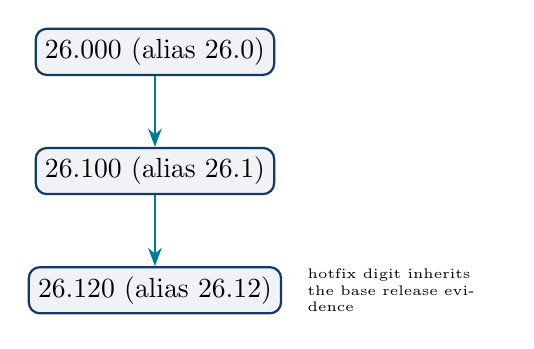
\begin{tikzpicture}[node distance=9mm]
      \node[draw=deepblue,thick,rounded corners,fill=softgray,minimum width=30mm] (a) {26.000 (alias 26.0)};
      \node[draw=deepblue,thick,rounded corners,fill=softgray,minimum width=30mm,below=of a] (b) {26.100 (alias 26.1)};
      \node[draw=deepblue,thick,rounded corners,fill=softgray,minimum width=30mm,below=of b] (c) {26.120 (alias 26.12)};
      \draw[-{Stealth},thick,accentteal] (a) -- (b);
      \draw[-{Stealth},thick,accentteal] (b) -- (c);
      \node[right=2mm of c,text width=24mm,font=\tiny] {hotfix digit inherits the base release evidence};
    \end{tikzpicture}
    \end{center}
  \end{columns}
\end{frame}

\begin{frame}{The command database and its four evidence statuses}
  \begin{columns}[T]
    \column{0.52\textwidth}
    \begin{itemize}
      \item 144 commands, one YAML file per manual chapter, loaded and validated at import.
      \item Every entry carries: layout grammar, emission phase, typed arguments, a manual page citation, and per-version evidence.
      \item Statuses are never hand edited: promotions happen only through committed probe reports.
    \end{itemize}
    \column{0.46\textwidth}
    \small
    \begin{tabular}{@{}ll@{}}
      \toprule
      Status & Meaning \\
      \midrule
      {\color{statusgreen}\textbf{documented}} & the manual says so \\
      {\color{statusblue}\textbf{verified}} & a probe passed on a real solver \\
      {\color{statusred}\textbf{broken}} & a probe contradicted the manual \\
      {\color{statusred}removed} & the manual states the removal \\
      \bottomrule
    \end{tabular}
    \vspace{2mm}
    \begin{block}{Honest emptiness}
      A version without recorded evidence shows an empty cell in the compatibility matrix, and the builder refuses it. No status is ever guessed.
    \end{block}
  \end{columns}
\end{frame}

\begin{frame}{The evidence lifecycle}
  \begin{center}
  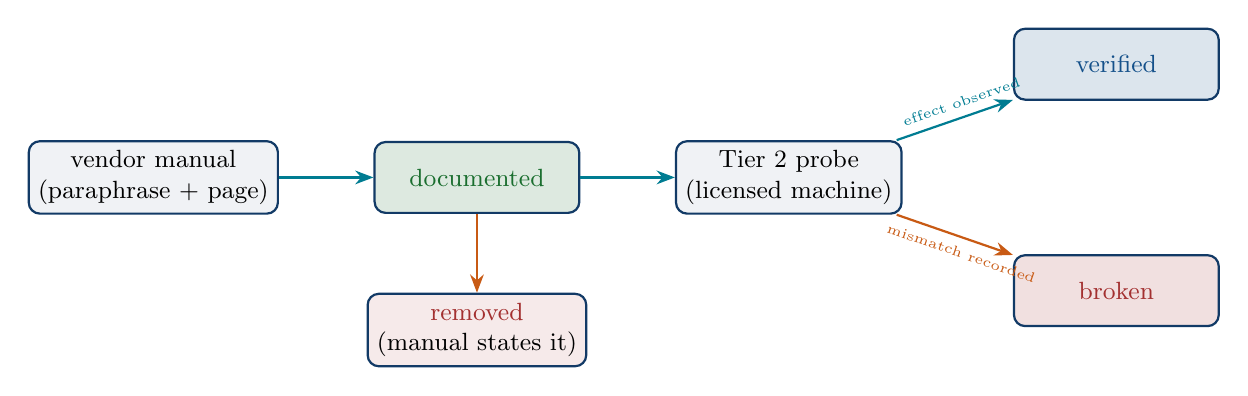
\begin{tikzpicture}[node distance=6mm and 12mm,
    box/.style={draw=deepblue,thick,rounded corners,fill=softgray,minimum width=26mm,minimum height=9mm,align=center,font=\small}]
    \node[box] (manual) {vendor manual\\(paraphrase + page)};
    \node[box,right=of manual,fill=statusgreen!15] (doc) {\color{statusgreen}documented};
    \node[box,right=of doc] (probe) {Tier 2 probe\\(licensed machine)};
    \node[box,above right=5mm and 14mm of probe,fill=statusblue!15] (ver) {\color{statusblue}verified};
    \node[box,below right=5mm and 14mm of probe,fill=statusred!15] (bro) {\color{statusred}broken};
    \node[box,below=10mm of doc,fill=statusred!10] (rem) {\color{statusred}removed\\(manual states it)};
    \draw[-{Stealth},thick,accentteal] (manual) -- (doc);
    \draw[-{Stealth},thick,accentteal] (doc) -- (probe);
    \draw[-{Stealth},thick,accentteal] (probe) -- (ver) node[pos=0.6,above,sloped,font=\tiny] {effect observed};
    \draw[-{Stealth},thick,accentorange] (probe) -- (bro) node[pos=0.6,below,sloped,font=\tiny] {mismatch recorded};
    \draw[-{Stealth},thick,accentorange] (doc) -- (rem);
  \end{tikzpicture}
  \end{center}
  \begin{center}
    \tiny promotion happens only through a committed compat report (pyfs-qa apply-compat)
  \end{center}
  \begin{itemize}
    \item Statuses are data with provenance: \code{verified} and \code{broken} entries cite the report file that proved them.
  \end{itemize}
\end{frame}

\begin{frame}{Three tiers of quality assurance behind the statuses}
  \small
  \begin{tabular}{@{}lllp{4.2cm}@{}}
    \toprule
    Tier & What it checks & Where it runs & Evidence artifact \\
    \midrule
    1 & schema, builder goldens, parsers & CI, no solver & green test suite (179 tests) \\
    2 & per-command validity probes & licensed machine & \code{reports/compat/} \\
    3 & physics regression and drift & licensed machine & \code{reports/physics/} \\
    \bottomrule
  \end{tabular}
  \vspace{3mm}
  \begin{itemize}
    \item Tier 2 asks: does this command do what the manual says, on this build? 65 commands verified and 3 found broken on 26.120.
    \item Tier 3 asks: does the physics still hold? A synthetic wing polar is anchored to finite-wing theory; a cross-version drift suite compares solver builds on identical inputs.
  \end{itemize}
\end{frame}

\begin{frame}{Takeaways: the mental model}
  \begin{block}{What to retain from this section}
    \begin{itemize}
      \item The FlightStream version is an input, canonical form \code{26.XXX}, ordered by an explicit list, never by number comparison.
      \item Every command the builder accepts is backed by evidence: a manual citation at minimum, a committed probe report at best.
      \item When the builder refuses, that refusal is the feature: it happens at build time, with the reason and the citation, instead of silently inside the solver.
    \end{itemize}
  \end{block}
\end{frame}

% =====================================================================
\section{Architecture}
% =====================================================================

\begin{frame}{The layered architecture}
  \begin{columns}[T]
    \column{0.5\textwidth}
    \begin{center}
    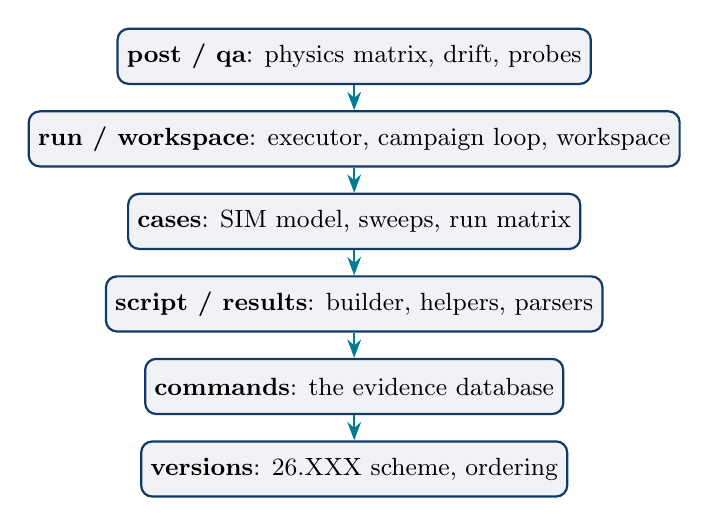
\begin{tikzpicture}[node distance=3.2mm,
      lay/.style={draw=deepblue,thick,rounded corners,fill=softgray,minimum width=46mm,minimum height=7mm,align=center,font=\small}]
      \node[lay] (qa) {\textbf{post / qa}: physics matrix, drift, probes};
      \node[lay,below=of qa] (run) {\textbf{run / workspace}: executor, campaign loop, workspace};
      \node[lay,below=of run] (cases) {\textbf{cases}: SIM model, sweeps, run matrix};
      \node[lay,below=of cases] (script) {\textbf{script / results}: builder, helpers, parsers};
      \node[lay,below=of script] (cmd) {\textbf{commands}: the evidence database};
      \node[lay,below=of cmd] (ver) {\textbf{versions}: 26.XXX scheme, ordering};
      \draw[-{Stealth},thick,accentteal] (qa) -- (run);
      \draw[-{Stealth},thick,accentteal] (run) -- (cases);
      \draw[-{Stealth},thick,accentteal] (cases) -- (script);
      \draw[-{Stealth},thick,accentteal] (script) -- (cmd);
      \draw[-{Stealth},thick,accentteal] (cmd) -- (ver);
    \end{tikzpicture}
    \end{center}
    \column{0.48\textwidth}
    \begin{itemize}
      \item Dependencies flow strictly downward; no layer imports upward.
      \item You can enter at any level of ambition:
      \begin{itemize}
        \item one validated script (\code{script}),
        \item one executed run (\code{run} + \code{results}),
        \item a whole campaign (\code{cases} + \code{workspace}).
      \end{itemize}
      \item The \code{qa} layer is how the library trusts itself; you rarely call it, but you benefit from every report it commits.
    \end{itemize}
  \end{columns}
\end{frame}

\begin{frame}{What each layer owns}
  \scriptsize
  \begin{tabular}{@{}lp{5.2cm}p{4.6cm}@{}}
    \toprule
    Layer & Owns & Key objects \\
    \midrule
    versions & canonical identifiers, ordering, aliases & \code{FsVersion}, \code{resolve}, \code{known\_versions} \\
    commands & per-version grammar and evidence & \code{CommandRegistry}, \code{CommandEntry} \\
    script & validating emission, phase order, layouts, helpers & \code{Script}, 16 curated helpers \\
    results & parsing solver output into typed reports & \code{parse\_loads}, \code{parse\_residual\_history} \\
    cases & what to run: SIM model, sweeps, recipes & \code{Campaign}, \code{SimCase}, \code{SweepAxis} \\
    workspace & managed run workspace and manifest & \code{CampaignWorkspace}, \code{RunRecord} \\
    run & how to run it: executor and campaign loop & \code{LocalExecutor}, \code{run\_campaign} \\
    qa & probes, physics matrix, drift, geometry & \code{pyfs-qa} CLI, \code{WingSpec} \\
    \bottomrule
  \end{tabular}
  \vspace{2mm}
  \begin{itemize}
    \item \code{post} (flow-visualization writers) and \code{fsi} (the aeroelastic coupling seam, behind the \code{[fsi]} extra) are delivered subpackages.
  \end{itemize}
\end{frame}

\begin{frame}{The script phase pipeline}
  \begin{center}
  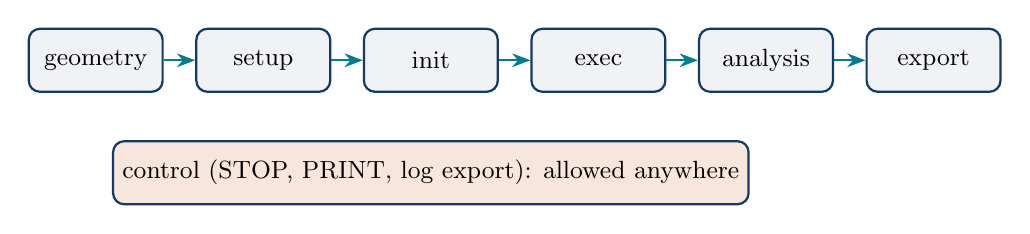
\begin{tikzpicture}[node distance=4mm,
    ph/.style={draw=deepblue,thick,rounded corners,fill=softgray,minimum width=17mm,minimum height=8mm,align=center,font=\small}]
    \node[ph] (g) {geometry};
    \node[ph,right=of g] (s) {setup};
    \node[ph,right=of s] (i) {init};
    \node[ph,right=of i] (e) {exec};
    \node[ph,right=of e] (a) {analysis};
    \node[ph,right=of a] (x) {export};
    \draw[-{Stealth},thick,accentteal] (g) -- (s);
    \draw[-{Stealth},thick,accentteal] (s) -- (i);
    \draw[-{Stealth},thick,accentteal] (i) -- (e);
    \draw[-{Stealth},thick,accentteal] (e) -- (a);
    \draw[-{Stealth},thick,accentteal] (a) -- (x);
    \node[ph,below=6mm of i,fill=accentorange!15,minimum width=40mm] (c) {control (STOP, PRINT, log export): allowed anywhere};
  \end{tikzpicture}
  \end{center}
  \begin{itemize}
    \item Every command in the database declares its phase. The builder tracks the highest phase reached and rejects a command whose phase precedes it.
    \item This encodes the manual's implicit ordering (import before initialize, initialize before solve) as an explicit, testable rule.
    \item The five layout grammars (bare, inline, param lines, payload lines, keyword block) are rendered for you; you never format a command line by hand.
  \end{itemize}
\end{frame}

% =====================================================================
\section{First Contact in Ten Minutes}
% =====================================================================

\begin{frame}[fragile]{Build a validated script}
\begin{lstlisting}
from pyflightstream.script import Script

script = Script(version="26.12")        # alias or canonical
script.comment("my first validated script")
script.emit("NEW_SIMULATION")
script.emit("IMPORT", "METER", "STL", "C:/work/wing.stl", clear=True)
script.emit("SET_SIMULATION_LENGTH_UNITS", "METER")
script.emit("AUTO_DETECT_TRAILING_EDGES")
text = script.render()                  # complete ASCII script
\end{lstlisting}
  \begin{itemize}
    \item \code{emit} validates the command name, the argument types and enum values, and the phase order, against the database view of the requested version.
    \item \code{render()} returns the exact text FlightStream will read; write it to a file when you are ready to execute.
  \end{itemize}
\end{frame}

\begin{frame}[fragile]{The errors are the teachers (1): typo and wrong value}
\begin{lstlisting}
script.emit("IMPRT", ...)
# CommandNotInVersionError: IMPRT is not in the command database.
# The database only holds commands drafted from the manual with
# citations; see CONTRIBUTING for how to add one.

script.emit("SET_SIMULATION_LENGTH_UNITS", "PARSEC")
# CommandArgumentError: names the argument, lists the allowed
# enum tokens, cites the manual page.
\end{lstlisting}
  \begin{block}{Design intent}
    Solver-side failures are silent or cryptic; the database knows enough to fail early. Every error message names the physical or version cause and carries a citation you can check.
  \end{block}
\end{frame}

\begin{frame}[fragile]{The errors are the teachers (2): version refusals}
\begin{lstlisting}[style=txt]
>>> Script(version="26.0").emit("NEW_SIMULATION")
CommandNotInVersionError: NEW_SIMULATION has no recorded evidence
for FlightStream 26.000. Recorded evidence: 26.100 (documented),
26.120 (verified). Earlier versions await release-notes review or
backfill probing.
\end{lstlisting}
  \begin{itemize}
    \item The refusal lists exactly what is known, per version, so you can decide: switch versions, or contribute the missing evidence.
    \item Removed commands explain themselves too: the removal note, the manual page, the last documented version, and the successor command when one is recorded.
  \end{itemize}
\end{frame}

\begin{frame}[fragile]{Execute and parse}
\begin{lstlisting}
from pathlib import Path
from pyflightstream.run import LocalExecutor
from pyflightstream.results import parse_loads

workdir = Path("C:/work/run1"); workdir.mkdir(exist_ok=True)
script_path = (workdir / "case.txt").resolve()   # absolute!
script_path.write_text(script.render(), encoding="utf-8")

executor = LocalExecutor("C:/FlightStream/FlightStream.exe")
result = executor.run_script(script_path, working_dir=workdir,
                             timeout_s=900.0)
if not result.failed:
    report = parse_loads((workdir / "loads.txt").read_text(),
                         requested_version="26.12")
    print(report.total["CL"], report.total["CDi"])
\end{lstlisting}
  \begin{itemize}
    \item \code{LocalExecutor} runs the documented headless invocation (\code{-hidden --script}, SRC-003 pp.279-280) with the working directory set for you.
  \end{itemize}
\end{frame}

\begin{frame}{Takeaways: first contact}
  \begin{block}{What to retain from this section}
    \begin{itemize}
      \item \code{Script(version=...)} then \code{emit(...)} then \code{render()}: three calls stand between you and a fully validated solver script.
      \item Make the script path and every imported geometry path absolute; the solver resolves relative paths against its own working directory (see the pitfalls section for the evidence).
      \item \code{ExecutionResult.failed} plus \code{parse\_loads} give you a typed, version-checked view of the run outcome.
    \end{itemize}
  \end{block}
\end{frame}

% =====================================================================
\section{The Curated Helpers}
% =====================================================================

\begin{frame}{Why helpers, and why only sixteen}
  \begin{columns}[T]
    \column{0.55\textwidth}
    \begin{itemize}
      \item The database records grammar; it cannot record conditionality written in manual prose (which extras each free-stream type takes, when the initializer takes per-surface lines).
      \item Helpers own exactly that conditional knowledge, as thin typed functions that only call \code{emit}: every line still passes database validation.
      \item One generated function per command was rejected by design: a huge surface that teaches nothing.
    \end{itemize}
    \column{0.43\textwidth}
    \small
    \begin{block}{The sixteen}
      free\_stream, atmosphere, solver\_settings, initialize\_solver, start\_solver, coordinate\_frame, sweep, analysis\_setup, export\_results, probe\_points, probe\_line, probes\_from\_file, export\_probes, actuator\_disc, rotary\_motion, unsteady\_solver
    \end{block}
  \end{columns}
\end{frame}

\begin{frame}[fragile]{Fluid state and free stream}
\begin{lstlisting}
from pyflightstream.script import helpers

# ISA sea level, explicit properties (the reliable path):
helpers.atmosphere(script, density=1.225, pressure=101325.0,
                   temperature=288.15, viscosity=1.7894e-05,
                   specific_heat_ratio=1.4)

helpers.free_stream(script)              # CONSTANT (default)
helpers.free_stream(script, "ROTATION",  # hover / rotor frames
                    frame=2, axis="X", rpm=2000.0)
\end{lstlisting}
  \begin{alertblock}{Why explicit properties}
    The altitude form (AIR\_ALTITUDE, SRC-003 p.328) was probed broken on 26.120: it applies feet regardless of the units argument (committed compat report). The helper still offers it, the matrix warns you, and this guide recommends FLUID\_PROPERTIES.
  \end{alertblock}
\end{frame}

\begin{frame}[fragile]{Solver settings and initialization}
\begin{lstlisting}
helpers.initialize_solver(script,
    solver_model="INCOMPRESSIBLE",   # or PRANDTL_GLAUERT, ...
    surfaces="all",
    wake_termination_x="DEFAULT",
    symmetry="NONE")                 # MIRROR, PERIODIC

helpers.solver_settings(script,
    aoa=4.0, velocity=30.0,
    ref_velocity=30.0, ref_area=8.0, ref_length=1.0,
    iterations=500, convergence=1e-5)
\end{lstlisting}
  \begin{itemize}
    \item \code{solver\_settings} emits only what you pass, so it serves both the initial setup and re-emission between campaign points.
    \item Reference area and length set the coefficient normalization ($Q\,S_{ref}$ forces, $Q\,S_{ref}\,L_{ref}$ moments; SRC-003 p.223).
  \end{itemize}
\end{frame}

\begin{frame}[fragile]{Analysis selection and exports}
\begin{lstlisting}
helpers.analysis_setup(script,
    load_units="COEFFICIENTS",
    vorticity_drag_boundaries="all")   # induced drag source

helpers.export_results(script,
    spreadsheet="loads.txt",           # the quantitative output
    vtk="surface.vtk", vtk_variables=["CP_REFERENCE"])
\end{lstlisting}
  \begin{itemize}
    \item Boundaries without trailing-edge boundary conditions silently report zero induced drag from the vorticity integration (SRC-003 p.202); select the drag boundaries deliberately.
    \item The plain \code{CP} export variable is flagged for depreciation (SRC-003 p.352); the helper warns and this guide uses \code{CP\_REFERENCE}.
  \end{itemize}
\end{frame}

\begin{frame}[fragile]{Probe management}
\begin{lstlisting}
helpers.probe_points(script, [(0.5, 0.0, 0.1),
                              (0.5, 0.5, 0.1)], units="METER")

helpers.probe_line(script, points=50, units="METER",
                   start=(1.5, 0.0, 0.0), end=(1.5, 4.0, 0.0))

helpers.probes_from_file(script, "lattice.csv", units="METER")

helpers.export_probes(script, "probes_out.txt", update=True)
\end{lstlisting}
  \begin{itemize}
    \item Probes are the flow-field window: velocities and pressures at chosen points, refreshed against the current solution before export.
    \item The file form takes X,Y,Z,TYPE rows (0 surface, 1 off body), for whole survey lattices (SRC-003 pp.362-363).
  \end{itemize}
\end{frame}

% =====================================================================
\section{Recipes: Step by Step per Simulation Type}
% =====================================================================

\begin{frame}{How the recipes are written}
  \begin{itemize}
    \item Each recipe lists: prerequisites, the numbered steps (geometry, script, run, parse), the expected outputs, and a pitfalls block.
    \item All scripts share the same skeleton; the recipes highlight only what changes.
    \item Every recipe was either executed on a real 26.120 build in the repository's QA history or is assembled from verified and documented commands with citations.
  \end{itemize}
  \begin{block}{The shared skeleton}
    NEW\_SIMULATION; IMPORT geometry; length units; trailing edge and wake auto-detect; fluid state; free stream; initialize; solver settings; START\_SOLVER; analysis selection; exports; CLOSE\_FLIGHTSTREAM.
  \end{block}
\end{frame}

% ---------------------------------------------------------------
\subsection{Recipe 1: steady single point}

\begin{frame}[fragile]{Recipe 1: steady single point (1/2)}
  \textbf{Prerequisites:} a surface mesh file (STL or another supported format) in known length units; the target FlightStream version; for execution, the licensed executable path.
  \begin{enumerate}
    \item Create the script and import the geometry:
  \end{enumerate}
\begin{lstlisting}
from pyflightstream.script import Script, helpers
script = Script(version="26.12")
script.emit("NEW_SIMULATION")
script.emit("IMPORT", "METER", "STL",
            str(stl_path.resolve()), clear=True)
script.emit("SET_SIMULATION_LENGTH_UNITS", "METER")
script.emit("AUTO_DETECT_TRAILING_EDGES")
script.emit("AUTO_DETECT_WAKE_TERMINATION_NODES")
\end{lstlisting}
  \begin{enumerate}
    \setcounter{enumi}{1}
    \item Set the fluid state and the free stream (previous section).
    \item Initialize with \code{symmetry="NONE"} and all surfaces.
  \end{enumerate}
\end{frame}

\begin{frame}[fragile]{Recipe 1: steady single point (2/2)}
  \begin{enumerate}
    \setcounter{enumi}{3}
    \item Solver settings: angle, velocity, references, iterations, convergence.
    \item \code{script.emit("START\_SOLVER")}.
    \item Analysis and export:
  \end{enumerate}
\begin{lstlisting}
helpers.analysis_setup(script, load_units="COEFFICIENTS",
                       vorticity_drag_boundaries="all")
helpers.export_results(script, spreadsheet="loads.txt")
script.emit("EXPORT_LOG", str((workdir / "log.txt").resolve()))
script.emit("CLOSE_FLIGHTSTREAM")
\end{lstlisting}
  \begin{enumerate}
    \setcounter{enumi}{6}
    \item Write, execute, parse (\code{LocalExecutor}, \code{parse\_loads}).
  \end{enumerate}
  \begin{alertblock}{Pitfalls}
    Geometry and script paths absolute. EXPORT\_LOG needs an absolute path (relative fails silently). Verify \code{report.current\_iteration < report.requested\_iterations} to confirm convergence rather than iteration exhaustion.
  \end{alertblock}
\end{frame}

% ---------------------------------------------------------------
\subsection{Recipe 2: steady polar (angle of attack sweep)}

\begin{frame}[fragile]{Recipe 2: steady polar, one script per point}
  \textbf{The proven pattern} (used by the repository's own physics QA): loop the single-point recipe over the angles, one script and one loads file per point.
\begin{lstlisting}
rows = []
for i, alpha in enumerate([-4, -2, 0, 2, 4, 6, 8]):
    script = build_point(version, alpha, f"loads_a{i}.txt")
    path = (workdir / f"polar_a{i}.txt").resolve()
    path.write_text(script.render(), encoding="utf-8")
    result = executor.run_script(path, working_dir=workdir)
    report = parse_loads((workdir / f"loads_a{i}.txt").read_text(),
                         requested_version=version)
    rows.append((alpha, report.total["CL"], report.total["CDi"]))
\end{lstlisting}
  \begin{itemize}
    \item Fully restartable: each point is independent evidence with its own log.
    \item This is exactly \code{examples/steady\_polar.py} in the repository, which also demonstrates the version refusal and the finite-wing sanity check.
  \end{itemize}
\end{frame}

\begin{frame}{Recipe 2: what a healthy polar looks like}
  \begin{columns}[T]
    \column{0.55\textwidth}
    \begin{center}
    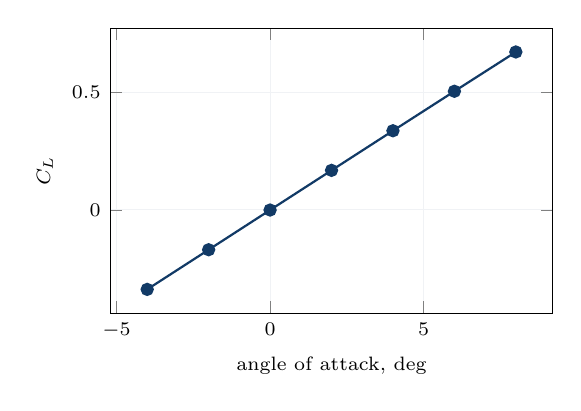
\begin{tikzpicture}
      \begin{axis}[width=72mm,height=52mm,
        xlabel={angle of attack, deg},ylabel={$C_L$},
        grid=both,grid style={softgray},
        tick label style={font=\scriptsize},
        label style={font=\scriptsize}]
        \addplot[color=deepblue,mark=*,thick] coordinates {
          (-4,-0.3382) (-2,-0.1694) (0,-0.0004)
          (2,0.1684) (4,0.3370) (6,0.5050) (8,0.6723)};
      \end{axis}
    \end{tikzpicture}
    \end{center}
    \column{0.43\textwidth}
    \begin{itemize}
      \item Real data: NACA 0012 rectangular wing, aspect ratio 8, FlightStream 26.120, from the committed example run.
      \item Lift slope 4.83 per rad; finite-wing theory anchor $2\pi/(1+2/AR) = 5.03$ per rad.
      \item A grossly wrong slope points at a broken import or symmetry setup, not at solver drift: cheap sanity first.
    \end{itemize}
  \end{columns}
\end{frame}

\begin{frame}[fragile]{Recipe 2 variant: the Sweeper Toolbox}
  \textbf{When to prefer it:} one solver session sweeping internally, reusing the solution between points (faster, but one shared session and one shared export).
\begin{lstlisting}
helpers.sweep(script,
    aoa=[-4.0, -2.0, 0.0, 2.0, 4.0, 6.0, 8.0],
    clear_solution=False,
    export_spreadsheet="sweep_results.txt")
\end{lstlisting}
  \begin{alertblock}{Pitfalls}
    The Sweeper chapter of the manual has not yet had its deep grammar review in the database (tracked follow-up); the drafted entries come from the worked example (SRC-003 p.406) and the script index (p.383). For evidence-critical campaigns, prefer one script per point.
  \end{alertblock}
\end{frame}

% ---------------------------------------------------------------
\subsection{Recipe 3: half model with mirror symmetry}

\begin{frame}[fragile]{Recipe 3: half model with MIRROR symmetry}
  \textbf{Prerequisites:} a true half geometry with an open root section lying in the symmetry plane. A face on the symmetry plane duplicates itself into coincident faces (SRC-003 p.386, paraphrased).
  \begin{enumerate}
    \item Import the half mesh; same skeleton as recipe 1.
    \item Initialize with mirror symmetry:
  \end{enumerate}
\begin{lstlisting}
helpers.initialize_solver(script, symmetry="MIRROR")
\end{lstlisting}
  \begin{enumerate}
    \setcounter{enumi}{2}
    \item Keep the FULL planform reference area, then request the symmetry loads explicitly:
  \end{enumerate}
\begin{lstlisting}
helpers.solver_settings(script, ref_area=full_planform_area, ...)
helpers.analysis_setup(script, symmetry_loads=True,
                       load_units="COEFFICIENTS")
\end{lstlisting}
  \begin{alertblock}{Pitfalls (all evidence backed)}
    Initializing MIRROR with a full model diverges instantly (SRC-003 p.217, paraphrased). The post-MIRROR symmetry loads default was calibrated on the real solver as ENABLE, but emit it explicitly: with DISABLE the loads halve and a one-wing rolling moment appears. Expected equivalence versus the full model: $\Delta C_L \approx +0.0015$, $\Delta C_{Di} = 0.0$ (committed physics report).
  \end{alertblock}
\end{frame}

% ---------------------------------------------------------------
\subsection{Recipe 4: actuator disc propulsion}

\begin{frame}[fragile]{Recipe 4: steady installed propulsion with an actuator disc (1/2)}
  \textbf{Concept:} the disc is the linearized propeller slipstream surrogate (SRC-003 pp.185-187); steady, cheap, no blade geometry.
  \begin{enumerate}
    \item Build the airframe skeleton as in recipe 1, up to the fluid state.
    \item Create a local coordinate system carrying the disc axis (frame index greater than 1):
  \end{enumerate}
\begin{lstlisting}
script.emit("CREATE_NEW_COORDINATE_SYSTEM")
script.emit("SET_COORDINATE_SYSTEM_ORIGIN", 2, x, y, z)
# orient axis as needed: SET_COORDINATE_SYSTEM_AXIS ...
\end{lstlisting}
  \begin{enumerate}
    \setcounter{enumi}{2}
    \item Create the disc through the helper (returns the actuator index):
  \end{enumerate}
\begin{lstlisting}
disc = helpers.actuator_disc(script, "prop1",
    frame=2, axis="X", offset=0.0,
    r_tip=0.95, r_hub=0.15, rpm=2200.0,
    thrust=850.0, thrust_type="NEWTONS")   # ELLIPTICAL model
\end{lstlisting}
\end{frame}

\begin{frame}[fragile]{Recipe 4: steady installed propulsion with an actuator disc (2/2)}
  \begin{enumerate}
    \setcounter{enumi}{3}
    \item Alternative thrust specification: a per-blade radial profile file (CUSTOM model), which then requires the blade count:
  \end{enumerate}
\begin{lstlisting}
disc = helpers.actuator_disc(script, "prop1",
    frame=2, axis="X", offset=0.0, r_tip=0.95, r_hub=0.15,
    rpm=2200.0, profile="radial_thrust.txt", n_blades=6,
    swirl=0.8)   # fraction of swirl kept; below 1 mimics a stator (SRC-003 p.186)
\end{lstlisting}
  \begin{enumerate}
    \setcounter{enumi}{4}
    \item Initialize, set solver settings, START\_SOLVER, analyze, export: identical to recipe 1.
  \end{enumerate}
  \begin{alertblock}{Pitfalls}
    Exactly one thrust specification: net thrust or profile, never both. The manual recommends dimensional thrust over the coefficient form, because the coefficient convention must match the solver formulation (SRC-003 p.187). The helper enforces both rules with cited errors.
  \end{alertblock}
\end{frame}

% ---------------------------------------------------------------
\subsection{Recipe 5: unsteady with resolved rotating blades}

\begin{frame}[fragile]{Recipe 5: unsteady rotary motion (1/2)}
  \textbf{Concept:} the blade-resolved alternative to the actuator disc (SRC-003 p.234): the blade geometry physically rotates through unsteady time stepping. Costlier, richer.
  \begin{enumerate}
    \item Import the full geometry including blades; identify the blade boundaries (their import order indexes them).
    \item Create the rotation frame (as in recipe 4), then the motion:
  \end{enumerate}
\begin{lstlisting}
motion = helpers.rotary_motion(script,
    frame=2, axis="X", rpm=2200.0,
    boundaries=[3, 4, 5, 6, 7, 8],   # the blade boundaries
    wake_stabilization_blades=6)
\end{lstlisting}
  \begin{enumerate}
    \setcounter{enumi}{2}
    \item Select the unsteady solver with the time step sized from the manual guidance: 8 to 12 degrees of blade rotation per step, at least two full rotations (SRC-003 p.210).
  \end{enumerate}
\begin{lstlisting}
# 2200 rpm = 13200 deg/s; 10 deg/step -> dt = 7.58e-4 s
# two rotations = 720 deg -> 72 steps
helpers.unsteady_solver(script, time_iterations=72,
                        delta_time=7.58e-4)
\end{lstlisting}
\end{frame}

\begin{frame}[fragile]{Recipe 5: unsteady rotary motion (2/2)}
  \begin{enumerate}
    \setcounter{enumi}{3}
    \item For rotor-dominated velocity scales, normalize with the tip speed instead of the free stream (SRC-003 p.201):
  \end{enumerate}
\begin{lstlisting}
tip_speed = 2200.0 / 60.0 * 2 * 3.14159 * r_tip
helpers.solver_settings(script, velocity=v_inf,
                        ref_velocity=tip_speed, ...)
\end{lstlisting}
  \begin{enumerate}
    \setcounter{enumi}{4}
    \item START\_SOLVER, then analysis and export as usual; the loads spreadsheet reflects the final time step.
  \end{enumerate}
  \begin{alertblock}{Pitfalls}
    SET\_MOTION\_START\_TIME was probed on 26.120 and found to abort scripts (committed compat report, broken status): converge the steady base flow by other means and treat the start-time argument with suspicion until re-probed. A positive start time is exactly the case the probe covered.
  \end{alertblock}
\end{frame}

% ---------------------------------------------------------------
\subsection{Recipe 6: probe surveys of the flow field}

\begin{frame}[fragile]{Recipe 6: probe surveys}
  \textbf{Concept:} extract velocities and pressures at chosen stations: wake rakes, slipstream surveys, control surfaces for conservation budgets.
  \begin{enumerate}
    \item Run any of recipes 1 to 5 up to and including START\_SOLVER.
    \item Define the stations (three equivalent entries):
  \end{enumerate}
\begin{lstlisting}
helpers.probe_points(script, [(1.5, 0.0, 0.0)], units="METER")
helpers.probe_line(script, points=50, units="METER",
                   start=(1.5, -2.0, 0.0), end=(1.5, 2.0, 0.0))
helpers.probes_from_file(script, "survey_lattice.csv",
                         units="METER")   # X,Y,Z,TYPE rows
\end{lstlisting}
  \begin{enumerate}
    \setcounter{enumi}{2}
    \item Export with refresh, so the values reflect the converged solution:
  \end{enumerate}
\begin{lstlisting}
helpers.export_probes(script, "probes_out.txt", update=True)
\end{lstlisting}
  \begin{alertblock}{Pitfalls}
    Keep \code{update=True} unless you deliberately want stale values; the export otherwise reflects whatever refresh happened last.
  \end{alertblock}
\end{frame}

% ---------------------------------------------------------------
\subsection{Recipe 7: batch campaigns}

\begin{frame}[fragile]{Recipe 7: campaigns (1/3), declare what to run}
  \textbf{Concept:} a campaign is data (TOML), a recipe is code (a function), the loop welds them with full provenance.
\begin{lstlisting}[style=txt]
[campaign]
name = "wing_steady_sweep"
fs_version = "26.12"
fs_exe = 'C:\FlightStream\26.12\FlightStream.exe'

[[sim]]
sim_id = "9001"
aircraft = "TestWing"
description = "steady polar"
reynolds = 4.38e6
mach = 0.1441
sweep = {type = "alpha", values = [-4.0, 0.0, 4.0, 8.0]}
recipe = "my_recipes:steady_point"
outputs = ["loads.txt"]
\end{lstlisting}
  \begin{itemize}
    \item Sweep axes: \code{alpha}, \code{beta}, \code{alpha\_beta} (pairs), \code{advance\_ratio}.
  \end{itemize}
\end{frame}

\begin{frame}[fragile]{Recipe 7: campaigns (2/3), write the recipe once}
\begin{lstlisting}
# my_recipes.py
from pyflightstream.cases import SimCase
from pyflightstream.script import Script, helpers

def steady_point(case: SimCase, script: Script) -> None:
    script.emit("NEW_SIMULATION")
    script.emit("IMPORT", "METER", "STL",
                str(case.staged_geometry), clear=True)
    ...  # skeleton as in recipe 1
    helpers.solver_settings(script,
        aoa=case.point["alpha"], ...)
    helpers.export_results(script, spreadsheet="loads.txt")
    script.emit("CLOSE_FLIGHTSTREAM")
\end{lstlisting}
  \begin{itemize}
    \item The loop fills \code{case.point} per sweep point and stages the geometry; output paths stay relative, so evidence lands inside the managed simulation folder.
    \item Recipes are imported functions, resolvable by name registry or \code{module:function} reference: explicit and versionable.
  \end{itemize}
\end{frame}

\begin{frame}[fragile]{Recipe 7: campaigns (3/3), run with provenance}
\begin{lstlisting}
from pyflightstream.cases import load_campaign
from pyflightstream.workspace import CampaignWorkspace
from pyflightstream.run import LocalExecutor, run_campaign
from pyflightstream.results import LoadsAssessor

campaign = load_campaign("campaign.toml")
records = run_campaign(campaign,
    executor=LocalExecutor(campaign.fs_exe),
    workspace=CampaignWorkspace("C:/work/campaign_root"),
    assess=LoadsAssessor())
\end{lstlisting}
  \begin{center}
  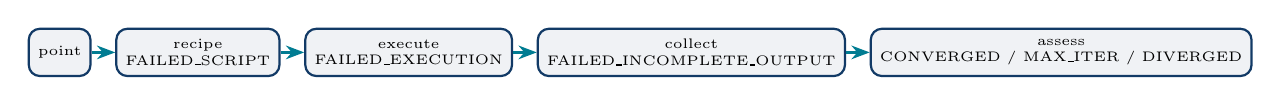
\begin{tikzpicture}[node distance=3mm,
    st/.style={draw=deepblue,thick,rounded corners,fill=softgray,minimum height=6mm,align=center,font=\tiny}]
    \node[st] (p) {point};
    \node[st,right=of p] (r) {recipe\\FAILED\_SCRIPT};
    \node[st,right=of r] (e) {execute\\FAILED\_EXECUTION};
    \node[st,right=of e] (c) {collect\\FAILED\_INCOMPLETE\_OUTPUT};
    \node[st,right=of c] (a) {assess\\CONVERGED / MAX\_ITER / DIVERGED};
    \draw[-{Stealth},thick,accentteal] (p) -- (r);
    \draw[-{Stealth},thick,accentteal] (r) -- (e);
    \draw[-{Stealth},thick,accentteal] (e) -- (c);
    \draw[-{Stealth},thick,accentteal] (c) -- (a);
  \end{tikzpicture}
  \end{center}
  \begin{itemize}
    \item Every executed point lands in exactly one of six statuses; a silent skip is structurally impossible. The manifest (\code{runs.json}, append only, with staging hashes) is the run identity: names lie, hashes do not.
  \end{itemize}
\end{frame}

\begin{frame}[fragile]{Recipe 7 addendum: migrating a run matrix}
  \begin{itemize}
    \item Coming from spreadsheet-driven run matrices (the pipe-delimited 15-column layout with AL and BE sweep codes)? The reader converts them losslessly:
  \end{itemize}
\begin{lstlisting}
from pyflightstream.cases.matrix import convert_matrix
text = convert_matrix("matrix.fs", name="wing2026",
    fs_version="26.120", fs_exe="C:/fs/FlightStream.exe",
    recipes={"003": "recipes.steady_polar:build"})
# the matrix codes are preserved as matrix_* variables,
# nothing is dropped; the TOML round-trips through load_campaign
\end{lstlisting}
  \begin{itemize}
    \item One-command form: the \code{pyfs-matrix convert} CLI takes the same inputs as flags and writes the file via \code{-o campaign.toml}.
    \item Convert once, review the TOML in a diff, then live natively in the campaign format.
  \end{itemize}
\end{frame}

\begin{frame}{Takeaways: choosing your recipe}
  \small
  \begin{tabular}{@{}lll@{}}
    \toprule
    You want & Recipe & Cost \\
    \midrule
    one force and moment set & 1: steady point & minutes \\
    a lift or drag polar & 2: polar (per point) & minutes per point \\
    symmetric config at half cost & 3: MIRROR half model & like 1 \\
    installed propulsion, steady & 4: actuator disc & like 1 \\
    blade-resolved slipstream & 5: unsteady rotary & hours \\
    flow-field quantities & 6: probes, on top of any & marginal \\
    hundreds of runs, provenance & 7: campaign & scales linearly \\
    \bottomrule
  \end{tabular}
  \vspace{2mm}
  \begin{block}{Composition}
    The recipes compose: a campaign whose recipe function builds an actuator disc case with a probe survey is just recipe 7 wrapping recipes 4 and 6.
  \end{block}
\end{frame}

% =====================================================================
\section{Reading Results}
% =====================================================================

\begin{frame}[fragile]{The loads report}
\begin{lstlisting}
report = parse_loads(text, requested_version="26.12")
report.total          # {"CL": ..., "CDi": ..., "CDo": ..., "CMy": ...}
report.surfaces       # per-boundary rows, keyed by name
report.current_iteration, report.requested_iterations
report.fs_version_reported, report.fs_build   # solver identity
\end{lstlisting}
  \begin{itemize}
    \item Convergence check: \code{current\_iteration < requested\_iterations} means the residual threshold was met before iteration exhaustion.
    \item The parser is strict about structure (a table without its closing Total row raises) and lax about version prefixes: the 26.120 build reports itself as "26.1", so the check records the reported string and build verbatim and warns on true mismatches.
  \end{itemize}
\end{frame}

\begin{frame}[fragile]{The residual history}
\begin{lstlisting}
from pyflightstream.results import parse_residual_history
samples = parse_residual_history(log_text)
# [ResidualSample(iteration=..., residual=...), ...]
\end{lstlisting}
  \begin{itemize}
    \item The residual trace is the difference between "it converged" and "it stopped": plot it when a result surprises you.
    \item Divergence shows as growth; a plateau above the threshold shows a case that needs more iterations or a better wake setup.
    \item The campaign assessor uses exactly these signals to separate CONVERGED from COMPLETED\_MAX\_ITER from FAILED\_DIVERGED.
  \end{itemize}
\end{frame}

% =====================================================================
\section{Versions and Evidence in Practice}
% =====================================================================

\begin{frame}{Reading the compatibility matrix}
  \begin{columns}[T]
    \column{0.55\textwidth}
    \begin{itemize}
      \item The docs site renders every command against every registered version; the same data backs \code{pyflightstream.help()}.
      \item Current evidence: 26.120 fully covered (65 {\color{statusblue}verified}, 74 {\color{statusgreen}documented}, 3 {\color{statusred}broken}, 2 removed); 26.100 partially backfilled (37 documented, 1 removed); 26.000 registered, honestly empty.
    \end{itemize}
    \column{0.43\textwidth}
    \begin{block}{When the builder refuses your version}
      \begin{enumerate}
        \item Check the matrix: is the command recorded for any version?
        \item If the manual for your version documents it, add the documented line with the page citation (contribution path).
        \item On a licensed machine, run the Tier 2 probe to promote it to verified.
      \end{enumerate}
    \end{block}
  \end{columns}
\end{frame}

\begin{frame}{Hotfix inheritance}
  \begin{itemize}
    \item A hotfix build (last canonical digit not zero) inherits the evidence record of its base release until probe evidence overrides it.
    \item Example: a future \code{26.121} would start from every \code{26.120} record; a probe on the hotfix build can then confirm or contradict each one.
    \item This keeps the honest default: a hotfix probably behaves like its base, but the moment evidence disagrees, the specific build gets its own record.
  \end{itemize}
  \begin{block}{Why the identifiers carry the hotfix digit}
    Vendor hotfix builds change solver behavior (this repository measured one: see the drift case study). They need identity in manifests and in the database.
  \end{block}
\end{frame}

% =====================================================================
\section{Real Solver Pitfalls, Evidence Backed}
% =====================================================================

\begin{frame}{Pitfalls found by the probe suite (Tier 2)}
  \small
  \begin{tabular}{@{}p{5.4cm}p{7.2cm}@{}}
    \toprule
    Finding & Practical rule \\
    \midrule
    AIR\_ALTITUDE ignores its units argument and applies feet & set the fluid state through FLUID\_PROPERTIES \\
    SET\_MOTION\_START\_TIME aborts the script & converge the base flow another way; await re-probe \\
    NEW\_OFF\_BODY\_STREAMLINE aborts the script & use probe lattices for off-body data \\
    \bottomrule
  \end{tabular}
  \vspace{2mm}
  \begin{itemize}
    \item All three carry {\color{statusred}\textbf{broken}} status in the database with the committed report cited; the builder still emits them (they are grammatically valid), but the matrix and the reference warn you. (NEW\_SURFACE\_SECTION\_DISTRIBUTION was in this list until the 2026-07-23 licensed re-probe promoted it to {\color{statusblue}\textbf{verified}} on the corrected phase and grammar.)
  \end{itemize}
\end{frame}

\begin{frame}{Pitfalls found by real runs (Tiers 2 and 3)}
  \begin{itemize}
    \item \textbf{Silent exit 0.} If \code{--script} names a missing file, the solver exits with code 0 and zero outputs. Always resolve the script path absolute, and treat "no outputs" as failure (the campaign loop does).
    \item \textbf{Relative paths resolve against the solver working directory.} Imported geometry: absolute. EXPORT\_LOG: absolute, or it fails silently.
    \item \textbf{The hidden solver idles after STOP.} A headless session that hits STOP does not exit; the executor's timeout is your safety net, and the log pair is the halt evidence.
    \item \textbf{Zero induced drag is not always good news.} Boundaries without trailing-edge boundary conditions report zero from the vorticity integration; select drag boundaries deliberately.
    \item \textbf{The transitional boundary layer model has a validity window.} Stated valid for chord Reynolds numbers between 500000 and 1500000 (SRC-003 p.203); outside it, select LAMINAR or TURBULENT explicitly.
  \end{itemize}
\end{frame}

% =====================================================================
\section{Where the Confidence Comes From}
% =====================================================================

\begin{frame}{The physics anchors}
  \begin{itemize}
    \item The committed physics matrix runs a synthetic NACA 0012 wing (generated from code, reproducible by anyone) against banded references:
    \begin{itemize}
      \item PHY-01, the polar: per-angle $C_L$, the lift slope against the finite-wing anchor, induced drag at the reference angle.
      \item PHY-02, the symmetry equivalence: the mirrored half model must reproduce the full-span coefficients on the same full planform reference.
    \end{itemize}
    \item References change only through a tool that demands a written reason, and a reference update never shares a commit with code changes.
    \item Repeat runs on the same build are bit identical; that is the baseline that makes drift detection meaningful.
  \end{itemize}
\end{frame}

\begin{frame}{Case study: catching a real solver change between builds}
  \begin{columns}[T]
    \column{0.55\textwidth}
    \begin{itemize}
      \item The cross-version drift suite ran identical inputs on build 5012026 (26.100) and build 7012026 (26.120).
      \item Every synthetic metric: zero delta. One local body case: pitching moment moved 0.8 percent.
      \item Triage: reruns bit identical on both builds (not noise), identical input file hash (not setup), single boundary (localized). Verdict: a deterministic solver-side change between builds.
    \end{itemize}
    \column{0.43\textwidth}
    \begin{block}{Why this matters to you}
      This is the exact failure mode the library exists for: two builds, same script, quietly different answers. The version-aware design turns it from a mystery into a measured, documented fact with a report you can cite.
    \end{block}
  \end{columns}
\end{frame}

% =====================================================================
\section{Extending and Reference Sheets}
% =====================================================================

\begin{frame}{Extending the library}
  \begin{itemize}
    \item \textbf{Add a command:} draft the YAML entry with the manual citation, typed arguments, layout, and phase; Tier 1 validates the schema; a probe spec promotes it later. The repository ships a guided workflow for this.
    \item \textbf{Onboard a new FlightStream version:} register it in the ordered list, backfill documented statuses from its manual with citations, then probe on a licensed machine.
    \item \textbf{Contribute a recipe:} recipes are plain functions; ship them with your project or propose the pattern for the docs.
  \end{itemize}
  \begin{block}{The rules that keep it trustworthy}
    No manual text is ever reproduced (paraphrase plus citation only). No status is hand edited. Supported versions are never dropped. Every example is synthetic and reproducible from code.
  \end{block}
\end{frame}

\begin{frame}{Cheat sheet: phases and layouts}
  \small
  \begin{columns}[T]
    \column{0.48\textwidth}
    \textbf{Phases, in order}
    \begin{enumerate}
      \item geometry (import, mesh operations)
      \item setup (fluid, free stream, actuators, motions)
      \item init (initialize, solver settings)
      \item exec (START\_SOLVER)
      \item analysis (loads selection)
      \item export (spreadsheets, fields, logs)
    \end{enumerate}
    control commands (STOP, PRINT, log export) may appear anywhere.
    \column{0.48\textwidth}
    \textbf{Layout grammars}
    \begin{itemize}
      \item bare: name alone
      \item inline: arguments on the command line
      \item param lines: KEY VALUE lines ended by a blank line
      \item payload lines: a count, then that many data lines
      \item keyword block: KEY VALUE lines until a terminator
    \end{itemize}
    The builder renders all five; you never format them by hand.
  \end{columns}
\end{frame}

\begin{frame}[fragile]{Cheat sheet: the four command-line tools}
\begin{lstlisting}[style=txt]
pyfs-qa probe            --version ... --fs-exe ...   # Tier 2 probes
pyfs-qa apply-compat     REPORT.yaml                  # promote statuses
pyfs-qa physics          --version ... --fs-exe ...   # Tier 3 matrix
pyfs-qa drift            --fs-exe 26.100=A.exe --fs-exe 26.120=B.exe
pyfs-qa cases                                         # print Tier 3 matrix
pyfs-qa update-reference --case ... --reason "..."    # guarded write
pyfs-workspace init      DIR                          # scaffold a workspace
pyfs-matrix convert      matrix.fs -o campaign.toml   # run matrix to campaign
pyfs-fsi                 (aeroelastic coupling executable)
\end{lstlisting}
  \begin{itemize}
    \item The \code{pyfs-qa} tools (and \code{pyfs-fsi}) require a licensed machine and write dated report pairs (markdown plus YAML) under \code{reports/}; \code{pyfs-qa cases} runs nothing.
    \item \code{pyfs-workspace} and \code{pyfs-matrix} run anywhere: they scaffold the workspace tree and turn a run matrix into a campaign.
    \item As a user you consume the licensed results through the matrix; you only run the licensed tools when contributing evidence.
  \end{itemize}
\end{frame}

\begin{frame}{Closing: the contract between you and the library}
  \begin{block}{The library promises}
    \begin{itemize}
      \item It will never emit a command it cannot back with evidence for your declared version.
      \item Every refusal explains itself with the cause and a citation.
      \item Every run under the campaign loop lands in exactly one recorded status with reproducible provenance.
    \end{itemize}
  \end{block}
  \begin{block}{You promise}
    \begin{itemize}
      \item The FlightStream version is declared, not assumed.
      \item Executable and geometry paths are explicit and absolute.
      \item When you meet undocumented solver behavior, it becomes a probe spec or an issue, so the next user inherits evidence instead of folklore.
    \end{itemize}
  \end{block}
\end{frame}

\end{document}
